\section{Experiment}

The benchmark comprises 12 tasks spanning six scientific categories, including scientific computing, machine learning, computer vision, medical image analysis, and drug discovery (Table~\ref{tab:task_list}). All benchmark data are collected from real experimental runs, with several tasks corresponding to configurations reported in published literature. The tasks cover both discrete and continuous search spaces and range from low- to high-dimensional settings. To simulate realistic user-system interaction, each task provides background information to the LLM to support intent interpretation. Most datasets are generated through systematic grid-based exploration, while LCBench and the Chagas EP20 drug discovery dataset are constructed from Bayesian optimization trajectories. LCBench is a widely used AutoML benchmark~\cite{zimmer2021auto}. All tasks are organized as YAML specifications containing metadata, task definitions, concise problem descriptions, search spaces, and trial records.
\subsection{Compared methods and evaluation setup}
We evaluate SelfAI across all 12 benchmark tasks and compare it with classical optimization methods, including grid search and the Tree Parzen Estimator (TPE) optimizer~\cite{optuna}, referred to as BS. To assess robustness across model families, we instantiate SelfAI with different language-model backbones, including OpenAI-o3~\cite{openai2023gpt}, Llama3.3~\cite{llama}, Qwen2.5~\cite{bai2023qwen}, and DeepSeek-R1~\cite{guo2025deepseek}. All methods are evaluated under identical computational settings. Reasoning traces are retained for analysis and reproducibility. For all trials, the random seed is fixed, and the temperature is set to zero. The detailed settings of the benchmark are available in the Supplementary Materials.

\begin{table}[h!]
\centering
\setlength{\tabcolsep}{4pt}
\renewcommand{\arraystretch}{1.2}
\caption{List of tasks in SelfAI with different hyperparameters for multiple tasks and datasets.}
\begin{tabular}{@{}lllcccc@{}}
\toprule
\textbf{Category} & \textbf{Method} & \textbf{Task} & \textbf{Dim} & \textbf{Count} & \textbf{Ref.} \\ 
\midrule
\multirow{1}{*}{Scientific Computing} & Tensor Network & Image Completion & 3 & 64 & \cite{tw} \\  
\hline
\multirow{3}{*}{Machine Learning} 
 & Random Forest & Pricing Prediction & 5 & 162 & \cite{boston} \\
 & LSTM & Sentiment Analysis & 2 & 20 & \cite{sentiment_analysis} \\ 
 & GraphSAGE & Node Classification & 22 & 25 & \cite{yan2023unreal} \\ 
 \hline
\multirow{5}{*}{Computer Vision} & SIREN & Image Denoising & 2 & 25 & \cite{sitzmann2020implicit} \\
 & SIREN & Image Segmentation & 2 & 25 & \cite{sitzmann2020implicit} \\
 & ResNet & Image Classification & 4 & 9 & \cite{resnet} \\ 
 & MAE & Image Classification & 2 & 20 & \cite{mae} \\ 
 & FashionMnist-NN & Image Classification & 5 & 2000 & \cite{zimmer2021auto} \\ 
\hline
\multirow{2}{*}{Medical Image Analysis} & nnUnet & BraTS~\cite{brats} & 3 & 18 & \cite{nnunet} \\
 & nnUnet-revisited & BTCV~\cite{btcv} & 5 & 19 & \cite{nnunet_revisit} \\
Drug Discovery & DNN & Bioactivity Prediction & 4 & 30 & \cite{korotcov2017comparison} \\
\bottomrule
\end{tabular}
\label{tab:task_list}
\end{table}


\begin{table}[h]
    \renewcommand\arraystretch{1.2}
    \setlength{\tabcolsep}{2pt}
    \centering
    \caption{Averaged performance comparison of SelfAI across different tasks.}
    \label{tab:hit}
    % \resizebox{\textwidth}{!}{
    \begin{tabular}{llccccccc}
    \toprule
    Solver & Score$\uparrow$ & $\text{AUP}_D\downarrow$ & Best-Time$\downarrow$ & Stop-Time$\downarrow$ & Best Result$\uparrow$ & Hit-Rate$\uparrow$ & Rank \\
    \midrule
    GS & 0.2453 & 1.0000 & 0.5094 & 1.0000 & 1.0000 & 1.0000 & 14 \\
    BS & 0.1927 & 0.8106 & 0.6265 & 0.9881 & 1.0000 & 1.0000 & 15 \\
     LLM & 0.3526 & 0.7638 & 0.2949 & 1.0000 & 1.0000 & 0.9286 & 13 \\
    LLM-ES & 0.5294 & 0.2349 & 0.4691 & 0.4582 & 0.9981 & 0.6429 & 3 \\
    \midrule
    % The following results are from selfai using different LLMs.
    Qwen2.5-7b      & 0.5562 & 0.2154 & 0.4805 & 0.3945 & 0.9957 & 0.7857 & 2 \\
    Qwen2.5-14b     & 0.5015 & 0.3310 & 0.4926 & 0.4997 & 0.9969 & 0.7857 & 5 \\
    Qwen2.5-32b     & 0.4287 & 0.4684 & 0.5252 & 0.6133 & 0.9972 & 0.7857 & 10 \\
    Qwen2.5-72b     & 0.4189 & 0.5358 & 0.4531 & 0.7087 & 0.9995 & 0.8571 & 11 \\
    DeepSeek-r1-7b  & 0.4769 & 0.1802 & 0.7020 & 0.3093 & 0.9927 & 0.5000 & 8 \\
    DeepSeek-r1-14b & 0.4793 & 0.3956 & 0.4953 & 0.5100 & 0.9948 & 0.7143 & 7 \\
    DeepSeek-r1-32b & 0.4989 & 0.3476 & 0.4535 & 0.5433 & 0.9933 & 0.7857 & 6 \\
    DeepSeek-r1-70b & 0.4556 & 0.3513 & 0.5392 & 0.5299 & 0.9962 & 0.7143 & 9 \\
    Llama3.3-70b    & 0.3625 & 0.5483 & 0.5099 & 0.7271 & 0.9683 & 0.7143 & 12 \\
    GPT4-o3-mini    & 0.6433 & 0.2259 & 0.3168 & 0.3961 & 0.9989 & 0.8571 & 1 \\
    GPT4-o3         & 0.5140 & 0.2284 & 0.5477 & 0.3961 & 0.9966 & 0.6429 & 4 \\
    \bottomrule
    \end{tabular}
    % }
\end{table}


\section{Evaluation}

To characterize efficiency-diversity trade-offs in long-horizon exploration, we propose four metrics: Score, $\text{AUP}_D$, $t_{\text{best}}$, and $t_{\text{stop}}$ (Fig.~\ref{fig:comparison}a), the details of which are described in Sect.~\ref{sec:evaluation_reasoning}. These metrics not only reflect final performance but also explicitly capture when high-quality solutions are discovered, how broadly the search space is explored, and how efficiently exploration is terminated. Score aggregates normalized improvement while penalizing both delayed discovery of optimal configurations and prolonged exploration after performance plateaus. $\text{AUP}_D$ (Area Under the Performance-Diversity Curve) quantifies the diversity of explored high-quality solutions and summarizes how performance gains are distributed along the discovery trajectory. The metrics $t_{\text{best}}$ and $t_{\text{stop}}$ denote the normalized time first to identify the best result and the time at which exploration terminates, respectively. An effective solver minimizes both quantities, achieving early discovery while avoiding unnecessary trials. In this framework, effective exploration strategies attain a high Score with a relatively low $\text{AUP}_D$, indicating efficient discovery with minimal wasted exploration. Detailed per-task comparisons of Score, $\text{AUP}_D$, $t_{\text{best}}$, and $t_{\text{stop}}$ are provided in the Supplementary Materials~\ref{sec:supp_details_benchmark}.



Across 12 heterogeneous tasks and language-model backbones (Supplementary Sect. ~\ref{sec:supp_details_benchmark}), these results demonstrate that SelfAI yields consistent trajectory-level benefits. SelfAI does not merely improve convergence accuracy but fundamentally reorganizes exploration dynamics in long-horizon scientific discovery.  By reallocating experimental effort away from diminishing-return regions toward structurally informative areas of the search space, SelfAI implements a policy-adaptive exploration strategy that aligns with identifiable principles of long-horizon scientific discovery.

\subsection{Emergent principles of long-horizon scientific discovery}
We further investigate whether long-horizon scientific discovery exhibits consistent, task-agnostic principles when guided by trajectory-aware reasoning. Fig.~\ref{fig:siren_surface} illustrates these trajectory-level dynamics in the hyperparameter search landscape for image segmentation using SIREN (Sect.~\ref{sec:case_studies}). From principles of long-horizon scientific discovery, trajectory-level dynamics follow a characteristic three-stage trajectory: rapid escape from low-efficiency regions, early concentration of effort in high-potential areas, and termination near the optimal configuration. This structured progression highlights the central role of strategic trial allocation and adaptive stopping in the efficiency of long-horizon exploration. 

Aggregated performance across tasks and domains reveals additional trajectory-level regularities (Fig.~\ref{fig:bar_score_aup}). Despite task-dependent variations in relative rankings (Supplementary Fig.~\ref{fig:rank_heatmap}), SelfAI consistently achieves high Scores while maintaining relatively low $\text{AUP}_D$ values across heterogeneous tasks and language-model backbones. These results indicate that efficient discovery trajectories can be organized according to shared principles that are not tied to any single task or domain. 

Model scale alone does not systematically improve long-horizon discovery behavior. Larger models often sustain prolonged exploration of alternative hypotheses, leading to delayed commitment and reduced adaptability under fixed experimental budgets. In contrast, small and mid-sized models often exhibit more stable cumulative progress, earlier concentration on informative regions, and more reliable stopping behavior. These observations show that baseline LLM solvers relying on exhaustive exploration without principled stopping often exhaust their search budgets (Fig.~\ref{fig:flowchart}). In contrast, SelfAI-enabled solvers achieve substantially higher hit rates while terminating exploration significantly earlier. Notably, final performance is often near saturation across methods, with the best results differing only marginally. Nevertheless, significant differences exist in performance and diversity metrics, revealing substantial differences in identifying high-quality configurations and effectiveness in avoiding redundant experiments.



\begin{figure*}[t]
    \centering
    \begin{tabular}{c}
        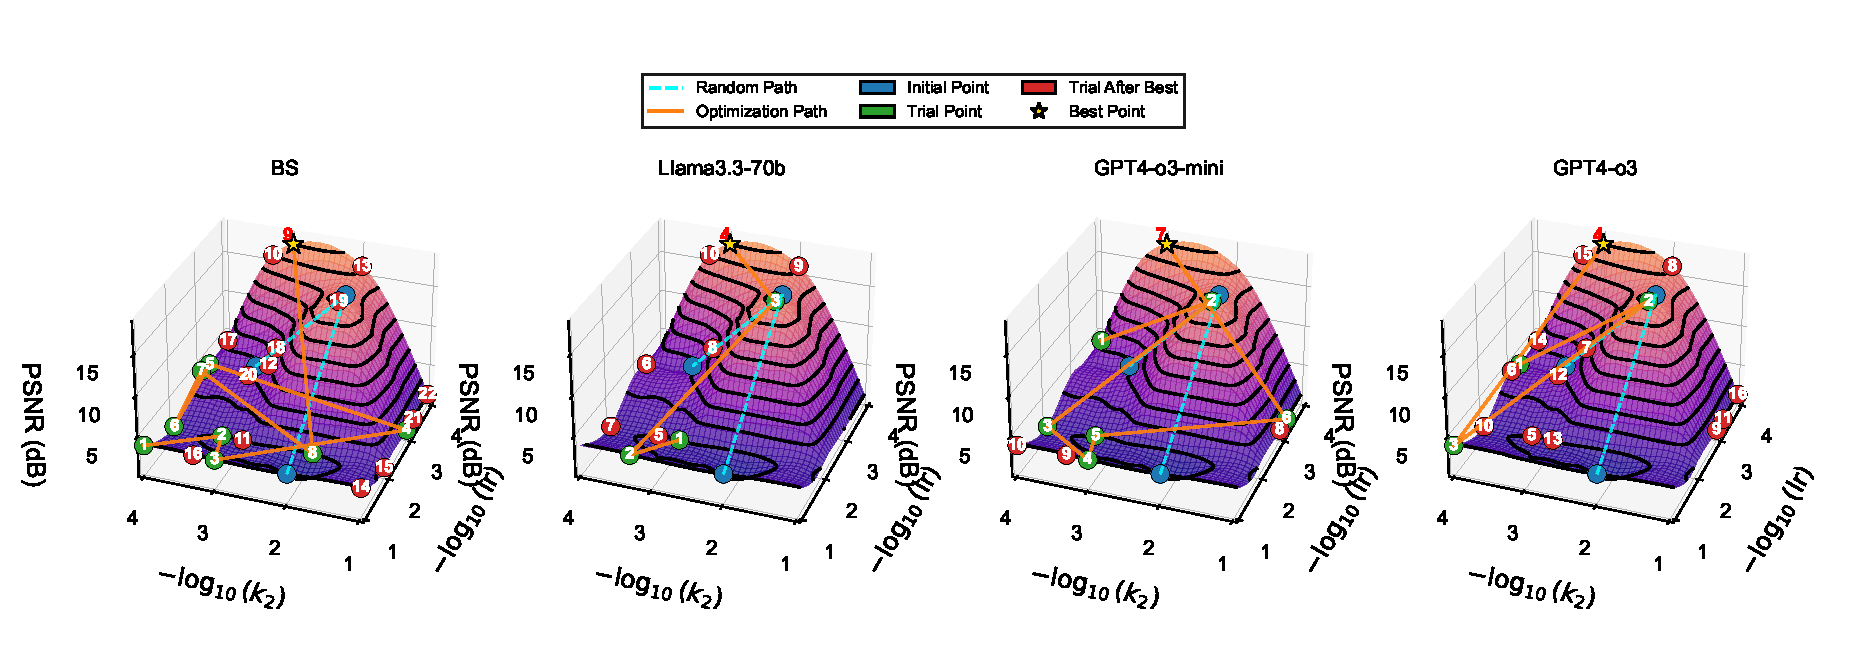
\includegraphics[width=1.0\textwidth]{figures/siren/cols/multi_model_comparison1.pdf} \\
        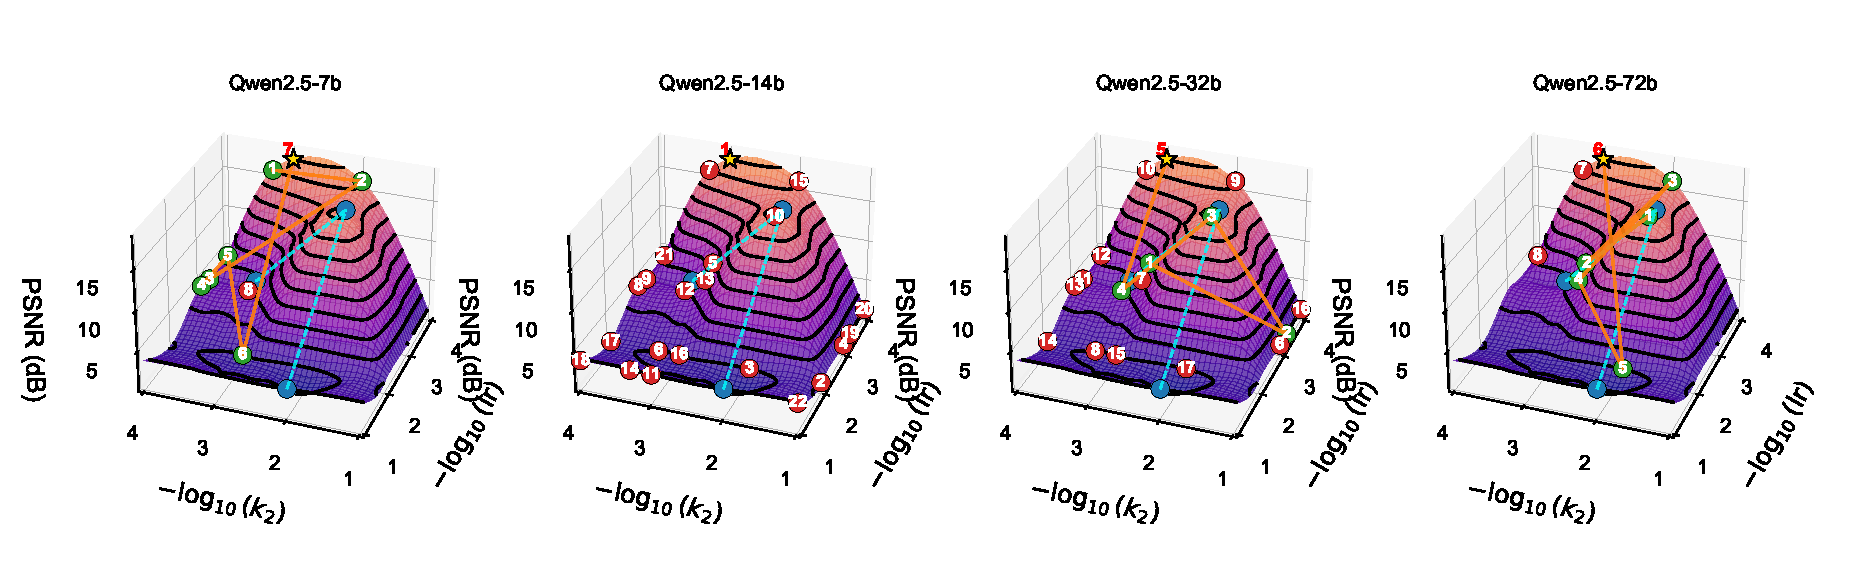
\includegraphics[width=1.0\textwidth]{figures/siren/cols/multi_model_comparison2.pdf} \\
        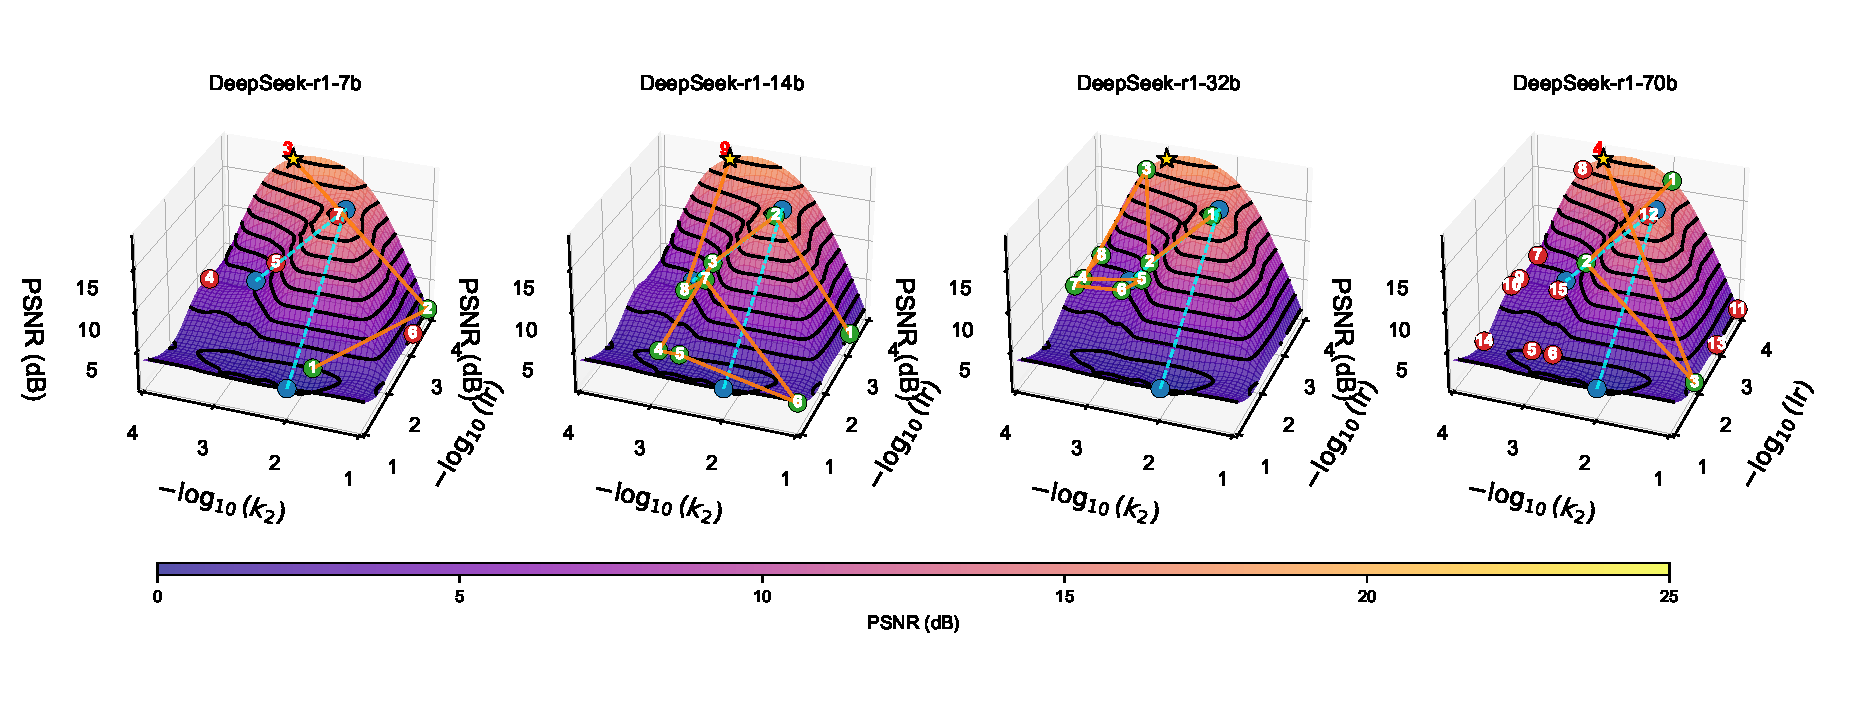
\includegraphics[width=1.0\textwidth]{figures/siren/cols/multi_model_comparison3.pdf} \\
    \end{tabular}
    \caption{Illustration of the optimized trajectory for the SIREN method for image segmentation. Green points are suggested points before reaching the optimal points. Red points are redundant suggestions when reaching out to the optimal points and failing to stop trials. The $\star$ is the optimal point. We show the serialization recommendations provided by LLM through the labeled numbers.}
    \label{fig:siren_surface}
\end{figure*}